
\def\tableconfiguration{ | p{4cm} | p{3cm} | p{3cm} | p{4cm} | }

\index{itk::Transform|textbf}

In the toolkit, \code{itk::Transform} objects encapsulate the mapping of points
and vectors from an input space to an output space.  If a transform is
invertible, back transform methods are also provided.  Currently, ITK provides
a variety of transforms from simple translation, rotation and scaling to
general affine and kernel transforms.  Note that, although we discuss
transforms in the context of registration in this section, transforms are
general and can be used for other applications. Some of the commonly used
transforms will be discussed in detail later in this section. Let's introduce
first the objects used in ITK for for representing basic spatial concepts.

\subsection{Geometrical Representation}
\label{sec:GeometricalObjects}

\begin{figure}
\center
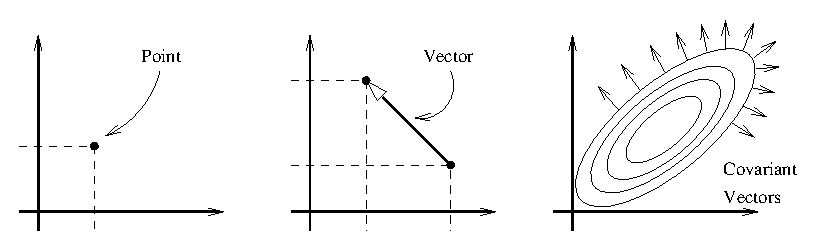
\includegraphics[width=14cm]{GeometricalObjects.eps}
\caption{Geometrical representation objects in ITK.}
\label{fig:GeometricalObjects}
\end{figure}
 
Insight implements a consitent geometric representation of the space. The
characteristics of classes involved in this representation are summarized in
the following table.

\index{itk::Point!Concept}
\index{itk::Vector!Concept}
\index{itk::CovariantVector!Concept}

\begin{center}
\begin{tabular}{ | p{4cm} | p{ 11cm } | }
\hline
\textbf{Class} &
\textbf{Geometrical concept} \\
\hline\hline
\code{itk::Point} & 
Position in space. In a $N$-Dimensional space it is represented by an array of
$N$ numbers associated with space coordinates. \\
\hline
\code{itk::Vector} & 
Relative position between two points. In a $N$-Dimensional space is represented
by an array of $N$-numbers each one associated with the distance along a
coordinate axis. Vectors do not have a position in space.\\
\hline
\code{itk::CovariantVector} & Orthogonal direction to a $(N-1)$-dimensional
manifold in space. For example, in $3D$ it corresponds to the vector orthogonal
to a surface. This is the apropriate class for representing gradients of
functions. Covariant vectors do not have a position in space.\\
\hline
\end{tabular}
\end{center}

Additional uses of the \code{Point}, \code{Vector} and \code{CovariantVector}
classes have been discussed in Chapter \ref{sec:DataRepresentation}.  Each one
of these classes behaves differently under spatial transformations. It is
henceforth quite important to keep their distinction clear. Figure
\ref{fig:GeometricalObjects} illustrates schematically the differences between
these concepts.


\index{itk::Transform!TransformPoint()}
\index{itk::Transform!TransformVector()}
\index{itk::Transform!TransformCovariantVector()}

\code{itk::Transform} classes provide different methods for mapping each one of
the basic space-representation object.  Points, vectors and covariant vectors
are transformed using the methods \code{TransformPoint()},
\code{TransformVector()} and \code{TransformCovariantVector()}.

\subsection{Transform General Properties}
\label{sec:TransformGeneralProperties}

\index{itk::Transform!SetParameters()}
Typically each transform type have several methods for setting its parameters.
For example, \code{Euler2DTransform} provide methods for separately setting the
offset, the angle, and the entire rotation matrix.  However, for use in the
registration framework, the parameters must also be represented by a flat
\code{Array<double>} to allow communication with generic optimizers. In the
case of \code{Euler2DTransform}, the transform is also defined by three
doubles: the first representing the angle and the last two the offset. The flat
array of parameters is defined using \code{SetParameters()}. A description of
the parameters and their ordering is documented in the following sections.
 
In the context of registration, the transform parameters define the search
space for optimizers. That is, the goal of the optimization is to find the
set of parameters defining a transform that optimizes the value of an image
metric. The more parameters a transform has, the longer its computational time
will be when used in a registration method since the dimension of the search
space will be equal to the number of transform parameters.

\index{itk::Transform!GetJacobian()}
Another requirement of the registration framework is the computation of the
transformation Jacobian. In general, metrics require the knowledge of the
Jacobian in order to compute the metric derivatives.  The Jacobian is a matrix
whose element are the partial derivatives of the output point with respect to
the array of parameters that defines the transform:

\begin{equation}
J=\left[ \begin{array}{cccc}
\frac{\partial x_{1}}{\partial p_{1}} & 
\frac{\partial x_{1}}{\partial p_{2}} & 
\cdots  & \frac{\partial x_{1}}{\partial p_{m}}\\
\frac{\partial x_{2}}{\partial p_{1}} & 
\frac{\partial x_{2}}{\partial p_{2}} & 
\cdots  & \frac{\partial x_{2}}{\partial p_{m}}\\
\vdots  & \vdots  & \ddots  & \vdots \\
\frac{\partial x_{n}}{\partial p_{1}} & 
\frac{\partial x_{n}}{\partial p_{2}} & 
\cdots  & \frac{\partial x_{n}}{\partial p_{m}}
\end{array}\right]
\end{equation}

Within this framework, the Jacobian is represented by a \code{Array2D<double>}
and is obtained from the transform by method \code{GetJacobian()}. The Jacobian
can be interpreted as a matrix that indicates for a point in the input space
how much its mapping on the output space will change as a response to a small
variation in one of the transform parameters. Note the the values of the
Jacobian matrix depend on the point in the input space. So actually the
Jacobian can be noted as $J(\bf{X})$. The use of transform Jacobians allows to
compute metric derivatives in a very efficient way. When Jacobians are not
available, metrics derivatives have to be computed using finite difference at a
price of $2M$ evaluations of the metric value, where $M$ is the number of
transform parameters.

The following sections describe the main characteristics of the transform
classes availables in ITK.

\subsection{Identity Transform}
\label{sec:IdentityTransform}

\begin{center}
\begin{tabular}{\tableconfiguration}
\hline
\textbf{Behavior} &
\textbf{Number of parameters} &
\textbf{Parameter Ordering} &
\textbf{Restrictions} \\
\hline\hline
Maps every point to itself, every vector to itself and every covariant vector to itself.  & 
0 &
  &  
Only defined when the input and output space has the same number of dimensions. \\
\hline
\end{tabular}
\end{center}

The identity transform is mainly used for debugging purposes. It is a mechanism
to provide a transform to methods that require it but yet have the certainty
that the transform will have no effect whatsoever in the outcome of the
process. It is just a \code{NULL} operation.


\subsection{Translation Transform}
\label{sec:TranslationTransform}

\begin{center}
\begin{tabular}{\tableconfiguration}
\hline
\textbf{Behavior} &
\textbf{Number of parameters} &
\textbf{Parameter Ordering} &
\textbf{Restrictions} \\
\hline\hline
Represents a simple translation of points in the input space
and has no effect on vectors or covariant vectors. &
Same as the input space dimension. &
The i-th parameter represents the translation in the i-th dimension. &
Only defined when the input and output space has the same number of dimensions. \\
\hline
\end{tabular}
\end{center}





\subsection{Scale Transform}
\label{sec:ScaleTransform}

\begin{center}
\begin{tabular}{\tableconfiguration}
\hline
\textbf{Behavior} &
\textbf{Number of parameters} &
\textbf{Parameter Ordering} &
\textbf{Restrictions} \\
\hline\hline
Represents a simple scaling of the vector space. Each component of a point, vector
or covariant vector is multiplied by the user defined scaling factor. &
Same as the input space dimension. &
The i-th parameter represents the scaling in the i-th dimension. &
Only defined when the input and output space has the same number of dimensions. \\
\hline
\end{tabular}
\end{center}





\subsection{Euler2DTransform}
\label{sec:Euler2DTransform}

\begin{center}
\begin{tabular}{\tableconfiguration}
\hline
\textbf{Behavior} &
\textbf{Number of parameters} &
\textbf{Parameter Ordering} &
\textbf{Restrictions} \\
\hline\hline
Represents a 2D rotation and a 2D translation. Note that the translation
component has no effect on the transformation of vectors and covariant vectors. &
3 &
The first parameter is the angle in radian and the last two parameters
are the translation in each dimension. &
Only defined for two-dimensional input and output spaces. \\
\hline
\end{tabular}
\end{center}





\subsection{Similarity2DTransform}
\label{sec:Similarity2DTransform}

\begin{center}
\begin{tabular}{\tableconfiguration}
\hline
\textbf{Behavior} &
\textbf{Number of parameters} &
\textbf{Parameter Ordering} &
\textbf{Restrictions} \\
\hline\hline
Represents a 2D rotation, homogeneous scaling and a 2D translation. Note that
the translation component has no effect on the transformation of vectors and
covariant vectors. & 
4 &
The first parameter is the angle in radian, the second the scaling factor for
all dimensions and the last two parameters are the translation in each
dimension. & 
Only defined for two-dimensional input and output spaces. \\
\hline
\end{tabular}
\end{center}


\subsection{QuaternionRigidTransform}
\label{sec:QuaternionRigidTransform}

\begin{center}
\begin{tabular}{\tableconfiguration}
\hline
\textbf{Behavior} &
\textbf{Number of parameters} &
\textbf{Parameter Ordering} &
\textbf{Restrictions} \\
\hline\hline
Represents a 3D rotation and a 3D translation. The rotation is specified as a
quaternion, defined by a vector of four numbers $\bf{q}$.  The relationship
between quaternion and rotation about vector $\bf{n}$ by angle $\theta$ is as
follows: \[ \bf{q} = (\bf{n}\sin(\theta/2), \cos(\theta/2))\] Note that if the
quaternion is not of unit length, scaling will also result. &
7 &
The first four parameters defines the quaternion and the last three parameters
the translation in each dimension. &
Only defined for three-dimensional input and output spaces. \\
\hline
\end{tabular}
\end{center}



\subsection{VersorRigid3DTransform}
\label{sec:VersorRigid3DTransform}


\begin{center}
\begin{tabular}{\tableconfiguration}
\hline
\textbf{Behavior} &
\textbf{Number of parameters} &
\textbf{Parameter Ordering} &
\textbf{Restrictions} \\
\hline\hline
Represents a 3D rotation and a 3D translation. The rotation is specified a
versor or unit quaternion, defined by a vector of three numbers.
These three numbers corresponds to the first three components of a quaternion.
The fourth component of the quaternion is derived such that the quaternion is of
unit length. &
6 &
The first three parameters defines the versor and the last three parameters the
translation in each dimension. &
Only defined for three-dimensional input and output spaces. \\
\hline
\end{tabular}
\end{center}



\subsection{AffineTransform}
\label{sec:AffineTransform}

\begin{center}
\begin{tabular}{\tableconfiguration}
\hline
\textbf{Behavior} &
\textbf{Number of parameters} &
\textbf{Parameter Ordering} &
\textbf{Restrictions} \\
\hline\hline
Represents an affine transform composed of rotation, scaling, shearing and
translation. The transform is specified by a $N \times N$ matrix and a $N
\times 1$ vector where $N$ is space dimension. &
$(N+1) \times N$ &
The first $N \times N$ parameters defines the matrix in column-major order
(where the column index varies the fastest).  The last $N$ parameters defines
the translate for each dimension. &
Only defined when the input and output space have the same dimension. \\
\hline
\end{tabular}
\end{center}





